%https://latexdraw.com/draw-flowcharts-latex-tutorial/

%https://tex.stackexchange.com/questions/8890/tikz-how-to-draw-boxes-around-set-of-nodes

%https://tikz.dev/tikz-shapes

%https://tex.stackexchange.com/questions/8890/tikz-how-to-draw-boxes-around-set-of-nodes

%https://www.latex4technics.com/?note=189T

\documentclass[border=0.2cm]{standalone}
 
% Required packages
\usepackage{comment}
\usepackage{tikz}
\usetikzlibrary{shapes,positioning,calc}


\usepackage{color}
\definecolor{franklinblue}{RGB}{0,43,83}
\definecolor{cardinalred}{RGB}{140,21,21}
\definecolor{skobeloff}{rgb}{0.0, 0.48, 0.45}
\definecolor{auburn}{rgb}{0.43, 0.21, 0.1}
\definecolor{calpolypomonagreen}{rgb}{0.12, 0.3, 0.17}
\definecolor{ao(english)}{rgb}{0.0, 0.5, 0.0}

\tikzset{
    ncbar angle/.initial=90,
    ncbar/.style={
        to path=(\tikztostart)
        -- ($(\tikztostart)!#1!\pgfkeysvalueof{/tikz/ncbar angle}:(\tikztotarget)$)
        -- ($(\tikztotarget)!($(\tikztostart)!#1!\pgfkeysvalueof{/tikz/ncbar angle}:(\tikztotarget)$)!\pgfkeysvalueof{/tikz/ncbar angle}:(\tikztostart)$)
        -- (\tikztotarget)
    },
    ncbar/.default=0.5cm,
}
\tikzset{square left brace/.style={ncbar=0.5cm}}
\tikzset{square right brace/.style={ncbar=-0.5cm}}
 
\begin{document}
 
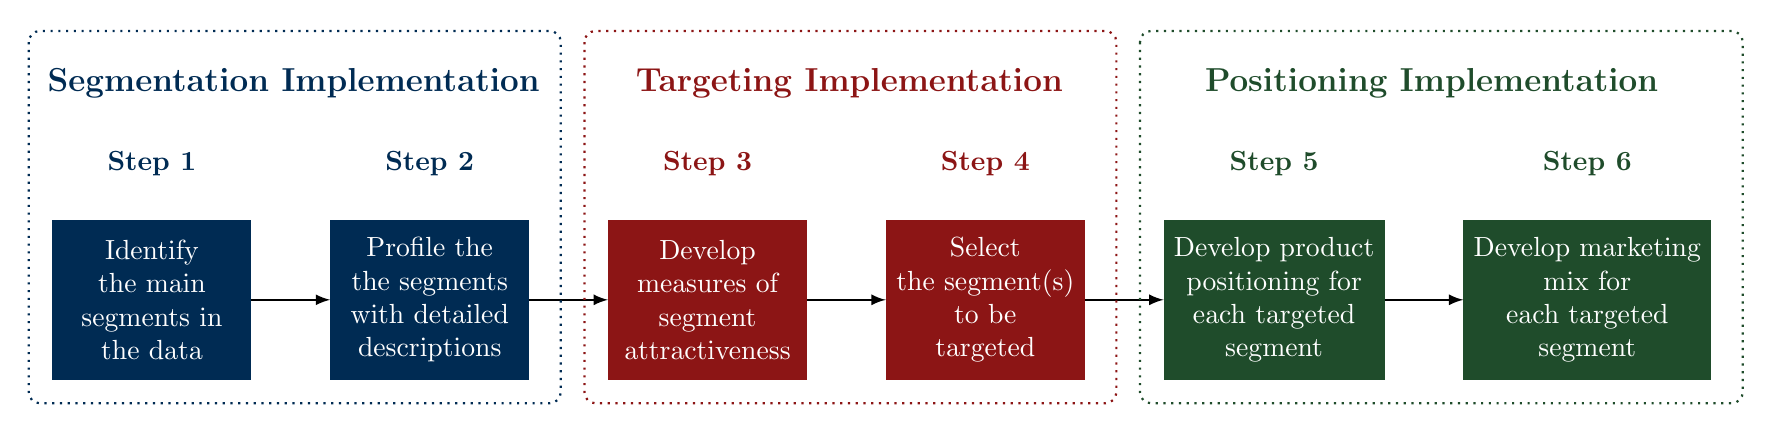
\begin{tikzpicture}[font=\normalsize,thick,align=center]
 
% Step 1
\node[draw=franklinblue,
    fill=franklinblue,
    text=white,
    rectangle,
    minimum width=2.5cm,
    minimum height=2.0cm] (block1) {Identify \\ the main \\ segments in \\ the data};

% Step 1 Marking
\node[text=franklinblue,
    above=of block1,
    yshift=-0.8cm,
    minimum width=2.5cm,
    minimum height=1.0cm] (block1A) {\textbf{Step 1}};

% Step 2
\node[draw=franklinblue,
    fill=franklinblue,
    text=white,
    rectangle,
    right=of block1,
    minimum width=2.5cm,
    minimum height=2.0cm] (block2) {Profile the \\ the segments \\ with detailed \\ descriptions};

% Step 2 Marking
\node[text=franklinblue,
    above=of block2,
    yshift=-0.8cm,
    minimum width=2.5cm,
    minimum height=1.0cm] (block2A) {\textbf{Step 2}};

% Steps 1 and 2 
\node[text=franklinblue,
    above=of block1A,
    yshift=-1.2cm,
    xshift=1.8cm,
    minimum width=2.5cm,
    minimum height=1.4cm] (block_1_2) {{\large \textbf{Segmentation Implementation}}};

% Step 3
\node[draw=cardinalred,
    fill=cardinalred,
    text=white,
    rectangle,
    right=of block2,
    minimum width=2.5cm,
    minimum height=2.0cm] (block3) {Develop \\ measures of \\ segment \\attractiveness};

% Step 3 Marking
\node[text=cardinalred,
    above=of block3,
    yshift=-0.8cm,
    minimum width=2.5cm,
    minimum height=1.0cm] (block3A) {\textbf{Step 3}};

% Step 4
\node[draw=cardinalred,
    fill=cardinalred,
    text=white,
    rectangle,
    right=of block3,
    minimum width=2.5cm,
    minimum height=2.0cm] (block4) {Select \\ the segment(s) \\ to be \\ targeted};

% Step 4 Marking
\node[text=cardinalred,
    above=of block4,
    yshift=-0.8cm,
    minimum width=2.5cm,
    minimum height=1.0cm] (block4A) {\textbf{Step 4}};

% Steps 3 and 4 
\node[text=cardinalred,
    above=of block3A,
    yshift=-1.2cm,
    xshift=1.8cm,
    minimum width=2.5cm,
    minimum height=1.4cm] (block_3_4) {{\large \textbf{Targeting Implementation}}};

% Step 5
\node[draw=calpolypomonagreen,
    fill=calpolypomonagreen,
    text=white,
    rectangle,
    right=of block4,
    minimum width=2.5cm,
    minimum height=2.0cm] (block5) {Develop product \\ positioning for \\ each targeted \\ segment};

% Step 5 Marking
\node[text=calpolypomonagreen,
    above=of block5,
    yshift=-0.8cm,
    minimum width=2.5cm,
    minimum height=1.0cm] (block5A) {\textbf{Step 5}};

% Step 6
\node[draw=calpolypomonagreen,
    fill=calpolypomonagreen,
    text=white,
    rectangle,
    right=of block5,
    minimum width=2.5cm,
    minimum height=2.0cm] (block6) {Develop marketing \\ mix for \\ each targeted \\ segment};

% Step 6 Marking
\node[text=calpolypomonagreen,
    above=of block6,
    yshift=-0.8cm,
    minimum width=2.5cm,
    minimum height=1.0cm] (block6A) {\textbf{Step 6}};

% Steps 5 and 6 
\node[text=calpolypomonagreen,
    above=of block5A,
    yshift=-1.2cm,
    xshift=2.0cm,
    minimum width=2.5cm,
    minimum height=1.4cm] (block_5_6) {{\large \textbf{Positioning Implementation}}};

% Arrows
\draw[-latex] (block1) edge (block2)
    (block2) edge (block3)
    (block3) edge (block4)
    (block4) edge (block5)
    (block5) edge (block6)
    ;

% Boxes around Nodes

\draw[franklinblue,thick,dotted, rounded corners] ($(block1.north west)+(-0.3,2.4)$)  rectangle ($(block2.south east)+(0.4,-0.3)$);

\draw[cardinalred,thick,dotted, rounded corners] ($(block3.north west)+(-0.3,2.4)$)  rectangle ($(block4.south east)+(0.4,-0.3)$);

\draw[calpolypomonagreen,thick,dotted, rounded corners] ($(block5.north west)+(-0.3,2.4)$)  rectangle ($(block6.south east)+(0.4,-0.3)$);



\end{tikzpicture}
 
\end{document}